\chapter{Implementation}
This section discusses the implementation of the music social network it is split into the multiple stories which have previously been listed.

\section{Story 1 - The Registration System}
\subsection{Back End}
Work began on the registration system by creating the appropriate tables on the back end. These tables were user\_types, users, genres and user\_genres. The user types table contained the three different types of account which a user could have: Music Lover, Artist and Venue Owner. The user type was done as a separate table to the users table itself for extensibility purposes as if additional user types needed to be added they could just simply be added to the table. The users table just contained all of the users details including name, display name, email, password (discussed in more depth during the security section) and a url link to there picture. The genres table was simply a table which contained different genre's of music and an appropriate id for each genre and as genres to users is a many to many relationship a users\_genres table was stored a user\_id and a genre\_id.

After the tables had been created the php files (hosted at seananderson.co.uk/api) were created. These php files essentially formed the RESTful API which would allow for the front end to connect to the database for the system. The first file which was created was register.php this file takes variables which the user passes in (through POST data) and adds them to the database via my sql commands which are ran from within the php. Some validation was done in the php file to check that things such as the email given are valid emails however I wanted to do most of the validation actually on the front end as this would allow for error messages to get out to the user quicker. 

As at this stage in time there was no front end it was not possible to test that sending post data from an app would work. So a piece of software called postman (which is a Google Chrome extension) was used as this software allows for post data to be pushed to a website as illustrated in figure X. As well as relying on the PHP file telling me 'A new user was added successfully' which is the message what is printed when the sql commands all run correctly the database was also checked to ensure that the new user had been added correctly as shown in figure X.

\begin{figure}[H]
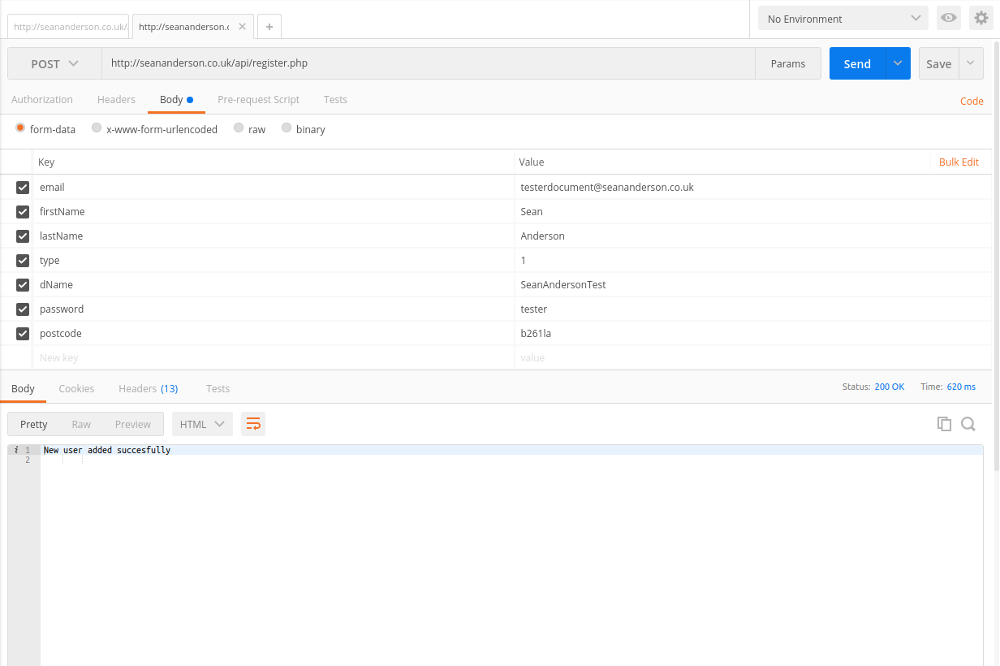
\includegraphics[scale=0.5]{images/postman}
\caption{Postman testing register.php}
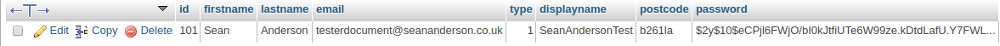
\includegraphics[scale=0.5]{images/db1}
\caption{User added to the database}
\end{figure}

For setting up registering different users genres the system was implemented in the exact same way as the registration system only that there was far fewer variables. The login API simply checks that the user provides an email and password and that they match and if they do match returns the user details and if they don't match returns a message saying that the password is not correct.

\subsubsection{Security within the Registration System}
It is important that users are not allowed to enter dangerous characters into the database, as a result of this all strings which will be imputed for the user (for all backend files for the music social media) are escaped using the mysqli\_escape function which is a default php function which ensures that any characters which could potentially do damage to the database are escaped and therefore not ran in the mysqli statements.

As the registration and login system used a password it was important to ensure that if somebody was to get access to the database that they wouldn't get access to the password. There are multiple different methods of encryption which could have been used for this. PHP has it's own built in function called password\_hash which takes in two parameters the password itself as a string and the encryption type. For this project password\_default which is a predefined php hashing method was used. Password default was used as it was a simplistic and relatively secure way of turning a password into a hash. The password\_verify function in PHP is used to check that a plain text password matches the hashed password.
 
\subsection{Front End}
After the back end for the registration of the app was created development then started on the front end of the app. The default ionic menu bar template was used as this would allow for a menu bar to appear on multiple pages (like in my design) easily.

The views for both the login and registration system were created using html (as are all views in ionic) and the controllers for those views were created in AngularJS and were simply js files. Both the register and login view files contained a form which gathered appropriate information from the user and then passed that information onto the controllers when submitted. The controllers then passed that information onto the API's by using \$http.post which is an AngularJS method used for calling post api's.

//TODO: Add sample code here.

In passing the information from the controller to the API I encountered a problem. AngularJS sends post data in a different way to most other languages. As a result of this the following lines of code had to be added to the PHP files. (This code was taken from \url{http://corpus.hubwiz.com/2/angularjs/15485354.html})
//TODO: Add code here.

Figure X shows what the front end for the login and registration screens look like on the front end on the system (from the perspective of a One Plus Two device.)

\begin{figure}[H]
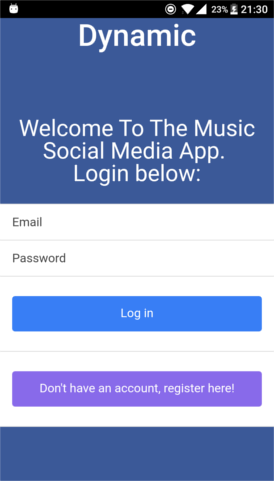
\includegraphics[scale=0.15]{images/sc1}
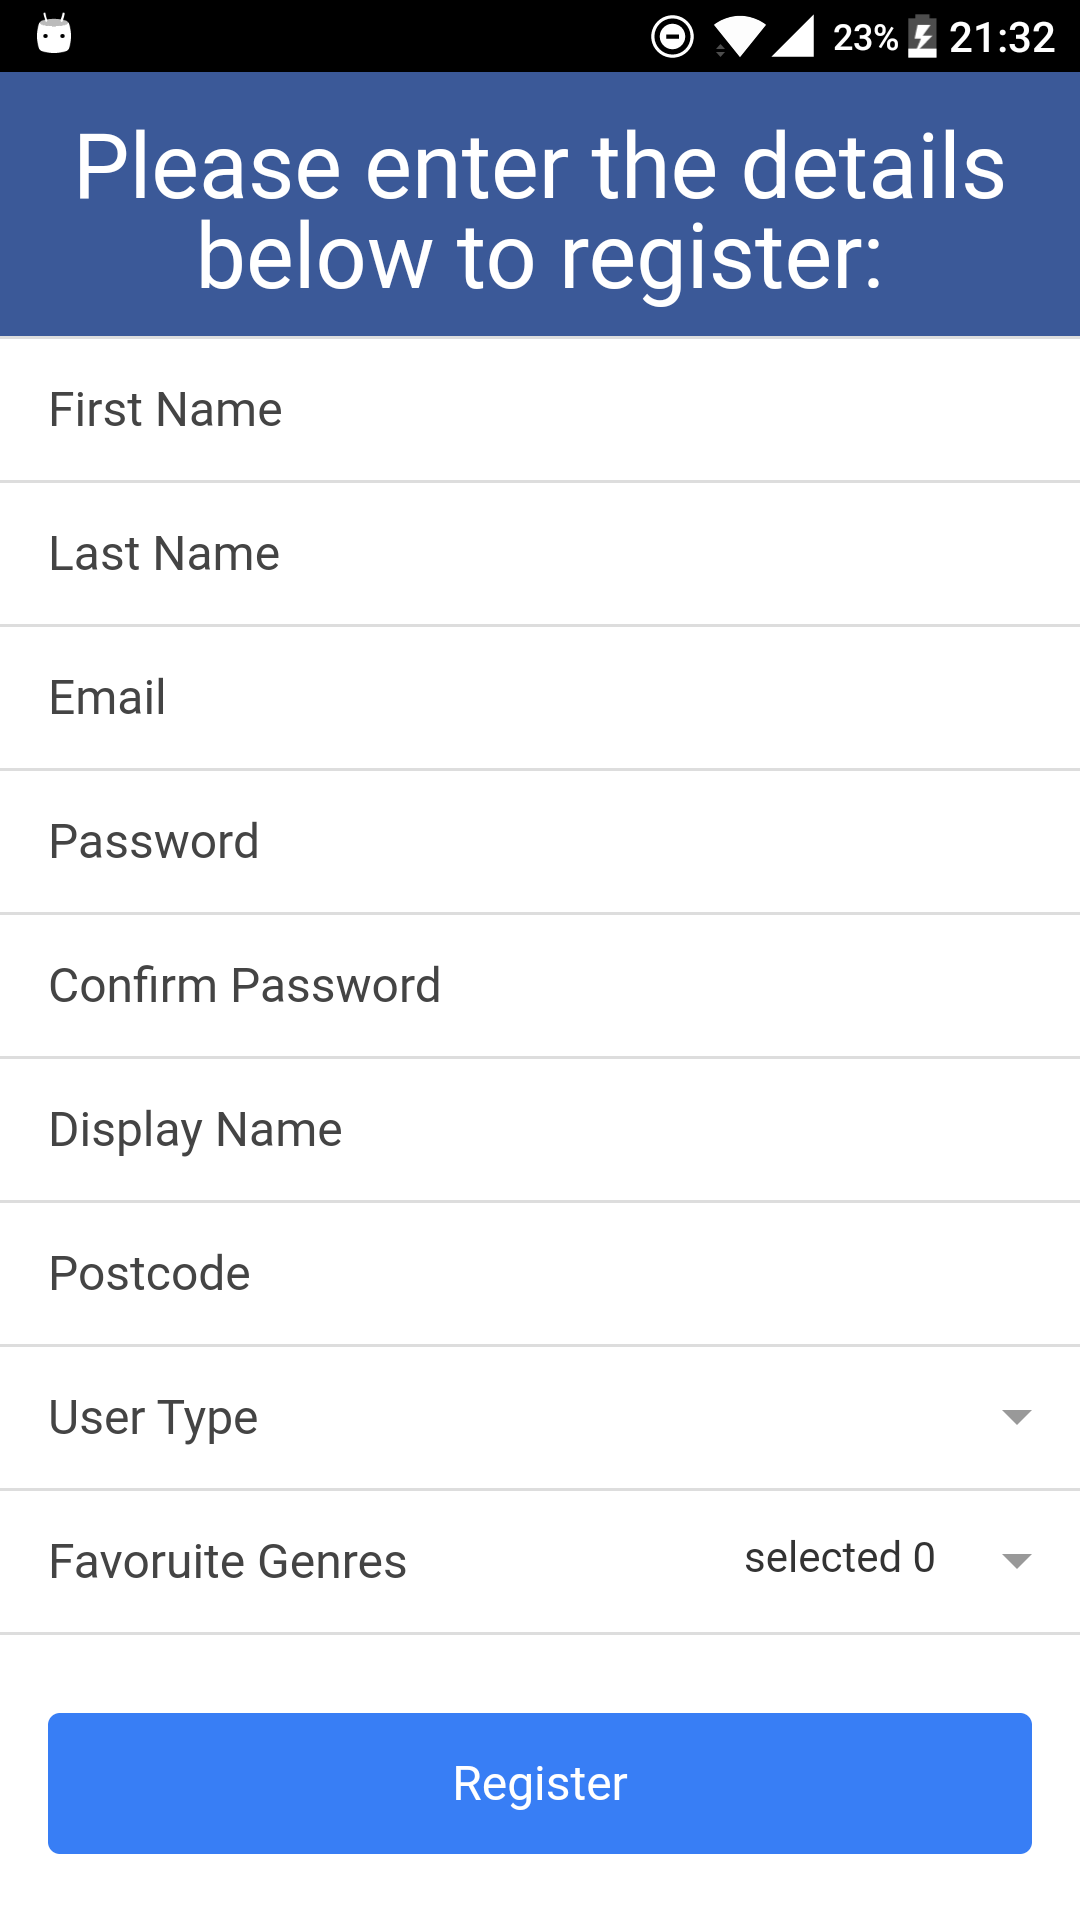
\includegraphics[scale=0.15]{images/sc2}
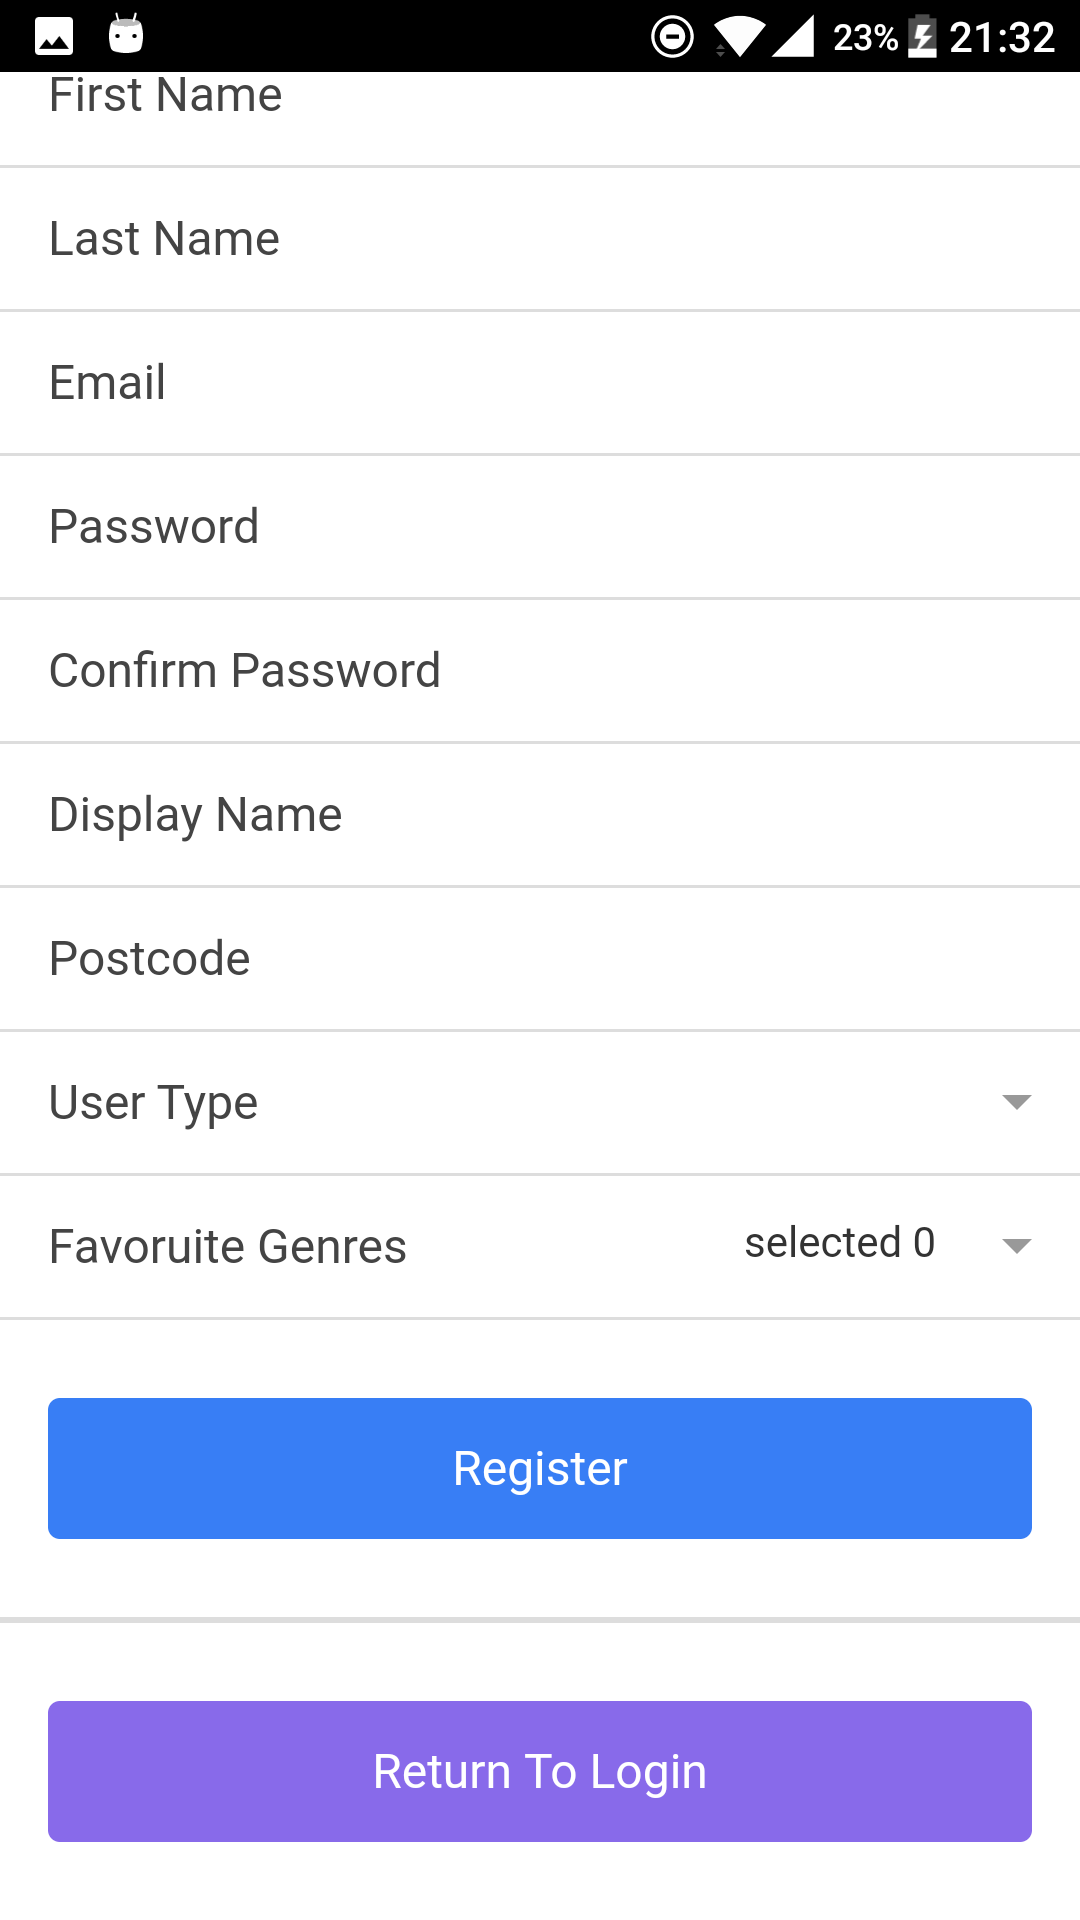
\includegraphics[scale=0.15]{images/sc3}
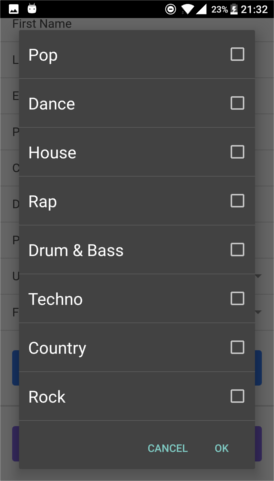
\includegraphics[scale=0.15]{images/sc4}
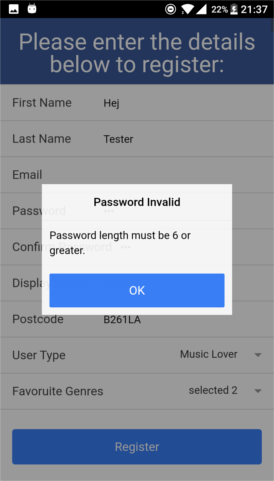
\includegraphics[scale=0.15]{images/sc5}
\caption{User added to the database}
\end{figure}

\subsection{Validation}
Having successfully got the front end interacting with the back end it was important to ensure that all of the data being sent over was valid. I decided first of all to validate the data on the front end so I ensured that the user had filled in all of the appropriate boxes and used a regex to ensure that the email address they entered was correct.

It was then necessary to create some more API files as each user had to have a unique email and display name files called checkemail.php and displayname.php were created these files run SQL queries to ensure that the email address and display name which the user entered are unique.

Figure X displays an example of what happens when a user tries to register an account with an email address which has already been used.



\section{Neil Info}

The implementation should look at any issues you encountered as you tried to implement your design. During the work, you might have found that elements of your design were unnecessary or overly complex; perhaps third party libraries were available that simplified some of the functions that you intended to implement. If things were easier in some areas, then how did you adapt your project to take account of your findings?

It is more likely that things were more complex than you first thought. In particular, were there any problems or difficulties that you found during implementation that you had to address? Did such problems simply delay you or were they more significant? 

You can conclude this section by reviewing the end of the implementation stage against the planned requirements. 
